\documentclass[main.tex]{subfiles}
% 向量函数及其图像
\begin{document}
在向量函数微积分部分的讨论,默认总是选择标准基作为$\mathbb{R}^n$的基,即,向量$\mathbf{f}=\left(f_1,\cdots,f_n\right)\in\mathbb{R}^n$的坐标就是$f_1,\cdots,f_n$,其矩阵是$\left(f_1,\cdots,f_n\right)^\intercal$。因此,是否把一个向量写成“列向量”(即$n\times 1$矩阵)的问题变得平凡。当我们想强调矩阵运算法则时,我们会注意明确“行、列向量”。我们会以专门的章节讨论选择非标准基乃至非规范正交基的情况。

\begin{definition}[向量函数]
从$\mathbb{R}^n$到$\mathbb{R}^m$的映射$\mathbf{f}:\mathbb{R}^n\rightarrow\mathbb{R}^m$是一个向量函数。其变量是一个$n$维向量空间的向量$\mathbf{r}\in\mathbb{R}^n$,$\mathbf{r}=\left(r_1,\cdots,r_n\right)$;其像(函数值)是一个$m$维向量空间的向量$\mathbf{f}\in\mathbb{R}^m$,$\mathbf{f}=\left(f_1,\cdots,f_m\right)$。在标准基下,$f_j:\mathbf{R}_n\rightarrow\mathbf{R},j=1,\cdots,m$称为$\mathbf{f}$的坐标函数。
\end{definition}

严格而言,函数的记法$\mathbf{f}:\mathbb{R}^n\supset D\rightarrow\mathbb{R}^m$表示函数$f$的定义域$\mathrm{dom}f=D$,而不是整个$\mathbf{R}^n$。这一记法中箭头右侧则一向仅指陪域。但是在后面的讨论当中,当定义域问题不重要时,我们也常粗略记为$\mathbf{f}:\mathbb{R}^n\rightarrow\mathbb{R}^m$。

\begin{example}
函数$\mathbf{f}:\mathbb{R}^3\rightarrow\mathbb{R}^2$,
\[\begin{split}\mathbf{f}\left(\mathbf{r}\right)=\left(\begin{array}{c}r_1^2+r_2^2+r_3^2\\r_1+r_2+r_3\end{array}\right)=\left(\begin{array}{c}f_1\\f_2\end{array}\right),\\f_1\leq0,f_2\in\mathbb{R}\end{split}\]
其中$\mathbf{r}=\left(r_1,r_2,r_3\right)^\intercal\in\mathbb{R}^3$,$\mathbf{f}=\left(f_1,f_2\right)^\intercal\in\mathbb{R}^2$。

以往我们更习惯把上述函数写成:
\[
\left\{\begin{array}{l}
    P\left(x,y,z\right)=x^2+y^2+z^2\\
    Q\left(x,y,z\right)=x+y+z
\end{array}
\right.
\]
\end{example}

\begin{example}
函数$\mathbf{f}:\mathbb{R}^3\rightarrow\mathbb{R}^2$,
\[\mathbf{f}\left(\mathbf{r}\right)=\left(\begin{array}{c}3r_1+4r_2\\3r_2+5r_3\end{array}\right)=\left(\begin{array}{ccc}3&4&0\\0&3&5\end{array}\right)\left(\begin{array}{c}r_1\\r_2\\r_3\end{array}\right)\]
是一个线性变换,又称线性函数。线性函数也可以按线性代数的惯例记为:$\mathbf{fr}$。
\end{example}

\begin{definition}[隐函数]
考虑函数$\mathbf{F}:\mathbb{R}^{n+m}\rightarrow\mathbb{R}^m$,若$\mathbb{R}^{n+m}$中的元素$\left(x_1,\cdots,x_n,y_1,\cdots,y_m\right)^\intercal$写成$\left(\mathbf{x},\mathbf{y}\right)^\intercal$,其中$\mathbf{x}=\left(x_1,\cdots,x_n\right)^\intercal$,$\mathbf{y}=\left(y_1,\cdots,y_m\right)^\intercal$,则$\mathbf{F}\left(\mathbf{r}\right),\mathbf{r}\in\mathbb{R}^{n+m}$也可写成$\mathbf{F}\left(\mathbf{x},\mathbf{y}\right)$。若函数$\mathbf{f}:\mathbb{R}^n\rightarrow\mathbb{R}^m$满足方程$\mathbf{F}\left(\mathbf{x},\mathbf{y}\right)=\mathbf{0},\forall\mathbf{x}\in\mathbb{R}^n$则称这一方程隐含地定义了函数$\mathbf{f}$。
\end{definition}

\begin{example}
设函数$F\left(x,y\right)=x^2+y^2-1=0$,则“$F\left(x,f\left(x\right)\right)=x^2+\left(f\left(x\right)\right)^2-1=0\forall x\in\mathrm{dom}f$”隐含地定义了以下任一函数:
\begin{align*}
    f_1\left(x\right)&=\sqrt{1-x^2},-1\leq x\leq 1\\
    f_2\left(x\right)&=-\sqrt{1-x^2},-1\leq x\leq 1\\
    f_3\left(x\right)&=\left\{\begin{array}{ll}
    \sqrt{1-x^2},&-\frac{1}{2}\leq x\leq 0\\
    -\sqrt{1-x^2},&0\leq x\leq 1
    \end{array}\right.
\end{align*}
\end{example}

\begin{definition}[函数的图像]\footnote{请复习高等数学相关内容\cite[\S 6.4~6.7]{华工高数2009上}。}
函数$\mathbf{f}:\mathbb{R}^n\rightarrow\mathbb{R}^m$的图像是指所有有序对$\left(\mathbf{r},\mathbf{f}\left(\mathbf{r}\right)\right)$的集合。
\end{definition}

图像的数学概念是一个集合,我们把图像画在纸上的方式是一种惯例。具体地,由定义,函数$\mathbf{f}:\mathbb{R}^n\rightarrow\mathbb{R}^m$的图像是由所有满足
\[
\left\{\begin{array}{c}y_1=f_1\left(r_1,\cdots,r_n\right)\\\vdots\\y_m=f_m\left(r_1,\cdots,r_n\right)\end{array}\right.
\]
的点$\left(x_1,\cdots,x_n,y_1,\cdots,y_m\right)$的集合(是$\mathbb{R}^{n+m}$的子集)。其中$f_1,\cdots,f_m$是$\mathbf{f}$的坐标函数。

我们只懂在纸上画出维数小于等于3的图形,即图上的任一点的坐标最多为3个实数。因此我们懂得在纸上画出的函数图像仅包括$n+m\leq3$的情况。

\begin{figure}[h]
    \centering
    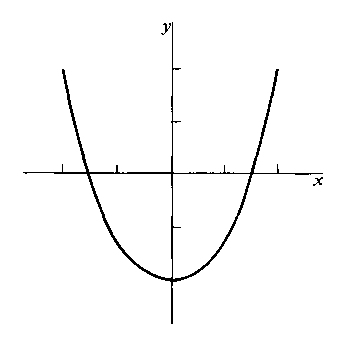
\includegraphics[width=0.5\textwidth]{images/II.10.1.eps}
    \caption{$y=x^2-2$}
    \label{fig:II.10.1}
\end{figure}

\begin{example}
函数$y=x^2-2$的图象是所有有序对$\left(x,y\right)$。同时,由于$\left(x,y\right)\in\mathbb{R}^2$,故这是平面上的图形。具体地,它是如图\ref{fig:II.10.1}所示的一条二次曲线。
\end{example}

\begin{figure}[h]
    \centering
    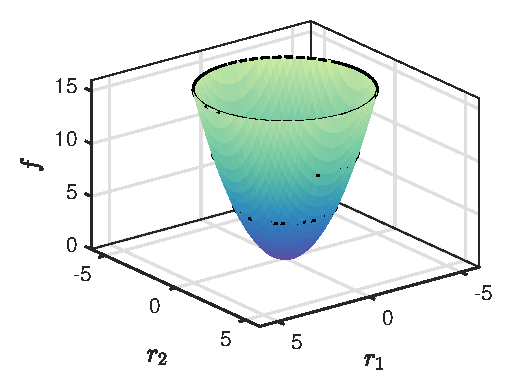
\includegraphics[width=0.5\textwidth]{images/II.10.2.eps}
    \caption{$f\left(\mathbf{r}\right)=\left\|\mathbf{r}\right\|^2$}
    \label{fig:II.10.2}
\end{figure}

\begin{example}\label{exp:II.12.5}
$f:\mathbb{R}^2\rightarrow\mathbb{R},f\left(\mathbf{r}\right)=\left\|\mathbf{r}\right\|^2$的图像是有序3元组$\left(r_1,r_2,f\right)$的集合,是3维空间的一个如图\ref{fig:II.10.2}所示的曲面。
\end{example}

\begin{figure}[h]
    \centering
    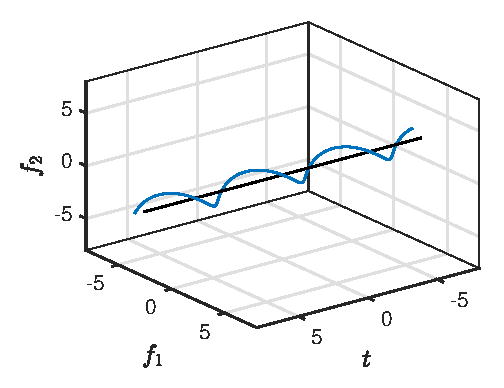
\includegraphics[width=0.5\textwidth]{images/II.10.3.eps}
    \caption{$\mathbf{f}\left(t\right)=\left(\cos t,\sin t\right)^\intercal$}
    \label{fig:II.10.3}
\end{figure}

\begin{example}\label{exp:II.12.6}
    函数$\mathbf{f}:\mathbb{R}\rightarrow\mathbb{R}^2$,
\[
\mathbf{f}\left(t\right)=\left(\begin{array}{c}\cos t\\\sin t\end{array}\right),t\in\mathbb{R}
\]
的图像是$\mathbb{R}^3$的子集。如何画出来?首先由函数定义式有$\left\|\mathbf{f}\left(t\right)\right\|=\sqrt{\cos^2t+\sin^2t}=1$,故$\mathbf{f}$的长度是恒定值。$t$是向量$\mathbf{f}$与$\mathbf{\hat{e}}_1$轴夹角的弧度。当$t$在$\mathbb{R}$内取不同值时,$\mathbf{f}$就在$\mathbf{\hat{e}}_1$-$\mathbf{\hat{e}}_2$平面上绕原点划出单位圆。但是,这个单位圆不是$\mathbf{f}$的图像。$\mathbf{f}$的图像是3元组$\left(t,\cos t,\sin t\right)$的集合,$\mathbb{R}^3$的子集,即如图\ref{fig:II.10.3}所示的螺线。
\end{example}

\begin{figure}[h]
    \centering
    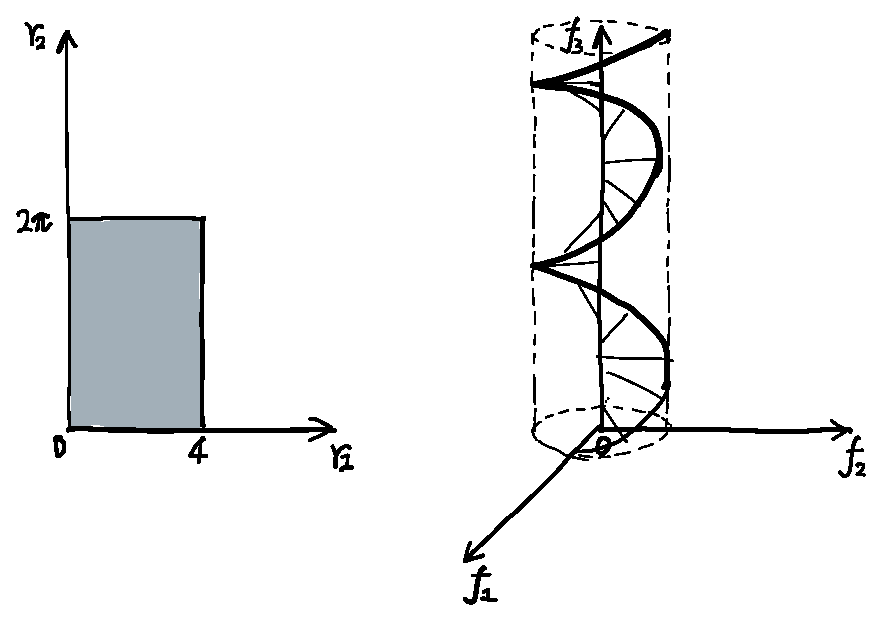
\includegraphics[width=0.5\textwidth]{images/II.10.4.eps}
    \caption{函数$\mathbf{f}\left(\mathbf{r}\right)=\left(f_1,f_2,f_3\right)\left(r_1\cos r_2, r_1\sin r_2,r_2\right)^\intercal,0\leq r_1\leq 4,0\leq r2\leq 2\pi$}
    \label{fig:II.10.4}
\end{figure}


\begin{example}
函数$f:\mathbb{R}^2\rightarrow\mathbb{R}^3,$
\[
\mathbf{f}\left(\mathbf{r}\right)=\left(\begin{array}{c}f_1\\f_2\\f_3\end{array}\right)=\left(\begin{array}{c}r_1\cos r_2\\r_1\sin r_2\\r_2\end{array}\right),0\leq r_1\leq 4,0\leq r_2\leq 2\pi
\]

$\mathbf{f}$的定义域是2维平面上的一个矩形(图\ref{fig:II.10.4})。令$r_1=a$,$a$是常数。则有
\[
\mathbf{f}=\left(\begin{array}{c}
    a\cos r_2\\
    a\sin r_2\\
    r_2
    \end{array}\right),0\leq r_2\leq 2\pi
\]
且$f_1^2+f_2^2=a^2$。把$r_2$作为$f_3$轴,则有序3元组$\left(a\cos r_2,a\sin r_2,r_2\right)$是一个螺线,其在$f_1-f_2$面上的投影是圆心在原点、半径为$a$的圆。令$r_2=\theta$,$\theta$是常数,则有
\[
\mathbf{f}=\left(\begin{array}{c}
    r_1\cos \theta\\
    r_1\sin \theta\\
    \theta
    \end{array}\right),0\leq r_2\leq 2\pi
\]
且$f_1^2+f_2^2=r_1^2$。在同样的空间坐标上,这是螺线上某点到$z$轴的线段。随着$a$在$\left[0,4\right]$上变化、$\theta$在$\left[0,2\pi\right]$上变化,以原函数$\mathbf{f}\left(\mathbf{r}\right)$的坐标函数为坐标的点集是如图\ref{fig:II.10.4}所示的螺带曲面。但按定义它不是函数$\mathbf{f}$的图像。我们说这个三维曲面是由一个参数方程$\mathbf{f}=\mathbf{f}\left(\mathbf{f}\right)$定义的曲面,它的参数$\mathbf{r}\in\mathbb{R}^2$域就是如图\ref{fig:II.10.4}所示的矩形区域,称为参数域。我们所画出来的3维曲面只是函数$\mathbf{f}$的值域。
\end{example}

\begin{definition}[函数的水平集]\footnote{在高等数学课里,我们学过水平集的概念\cite[\S7.1,p~1] {华工高数2009下}。}
函数$\mathbf{f}:\mathbb{R}^n\rightarrow\mathbb{R}^m$的水平集$S=\left\{\mathbf{r}|\mathbf{f}\left(\mathbf{r}\right)=\mathbf{a}\right\},\mathbf{a}\in\mathbb{R}^m$。
\end{definition}

\begin{figure}[h]
    \centering
    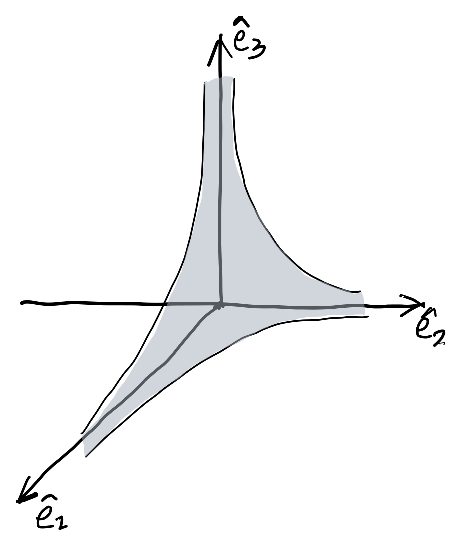
\includegraphics[width=0.25\textwidth]{images/II.10.5.eps}
    \caption{函数$f\left(\mathbf{r}\right)=r_1r_2+r_2r_3+r_3r_1$}
    \label{fig:II.10.5}
\end{figure}

\begin{example}\label{exp:II.12.8}
设函数$f:\mathbb{R}^3\rightarrow\mathbb{R},f\left(\mathbf{r}\right)=r_1r_2+r_2r_3+r_3r_1$及其一个水平集$S=\left\{\mathbf{r}|f\left(\mathbf{r}\right)=1\right\}$。以$S$的元素$\left(r_1,r_2,r_3\right)$为坐标的点集构成的三维图形是怎样的?设$r_3=0$得到方程$r_1r_2=1$,这定义了$\mathbf{\hat{e}}_1$-$\mathbf{\hat{e}}_2$平面上的一条双曲线,这条双曲线是$S$的图像与$\mathbf{\hat{e}}_1$-$\mathbf{\hat{e}}_2$平面的截线。类似地,$S$与$\mathbf{\hat{e}}_2$-$\mathbf{\hat{e}}_3$、$\mathbf{\hat{e}}_1$-$\mathbf{\hat{e}}_3$平面的截线也是类似的双曲线。更一般地,$S$是一个由一系列双曲线构成的曲面(如图\ref{fig:II.10.5}所示)。但是,按定义,这不是函
数$\mathbf{f}$的图像。
\end{example}

总结以上例子,我们给一个函数画出来的图有以下三种情况:

\begin{enumerate}
\item 如果$\mathbb{R}^{n+m}$的子集$S$是函数$\mathbf{f}:\mathbb{R}^n\rightarrow\mathbb{R}^m$的图像,则称$S$是由显函数定义的图像。
\item 如果$\mathbb{R}^{m}$的子集$S$是函数$\mathbf{f}:\mathbb{R}^n\rightarrow\mathbb{R}^m$的值域,则$S$是由参数方程定义的图像。
\item 如果$S$是函数$\mathbf{f}:\mathbb{R}^n\rightarrow\mathbb{R}^m$的一个水平集,则$S$是由隐函数定义的图像。
\end{enumerate}

注意:只有第1种情况中$S$才是函数$\mathbf{f}$的图像,但我们经常通过第2、3种情况中的$S$来认识函数$\mathbf{f}$。
\end{document}